
\subsection{Explore novel circuit techniques for NVM}

The advent of novel materials and devices have introduced a number of new design issues. On one hand, all types of emerging NVM technologies are facing to the common requirements -- fast speed, high density, affordable yield, low power, etc. On the other hand, the primary concern and effective solution could be quite different for each NVM technique because of the specific device characteristic and process integration difficulty. Our task here is to investigate the common design issues and to exploit distinctive circuit techniques for each individual emerging NVM technology. More specifically, we will focus on three main issues in memory design -- yield, reliability, and density.

\subsubsection{Write Endurance Improvement}

Write endurance is one of the biggest obstacles that prevent the emerging NVMs from massive production and wide application, although the physical mechanisms behind for various emerging NVMs are different. For PCRAM, writing is the primary wear mechanism: when injecting current into a volume of phase change material, thermal expansion and contraction degrades the electrode-storage contact~\cite{Lee09}. While in MRAM, the cell damage during write operations mainly is triggered by particles and pin-holes introduced in process integration.  Write endurance is usually measured as the number of writes performed before the cell cannot be programmed reliably. SRAM and DRAM both have endurance of about $10^{16}$ programming cycles~\cite{ITRS07}, which are sufficient for use even in high-performance processing. The best reported write endurance for PCRAM, however, is only 10$^9$ based on a survey of PCRAM device and circuit prototypes published within the last five years~\cite{Lee09}. And the best endurance test result of STT-RAM is less than $4\times10^{12}$ programming cycles~\cite{Diao07}.

Besides the improvements on device material and process development, the most straightforward and effective approach is to reduce the time period that writing current applied on the memory cell. Some architectural level solutions have been proposed previously, such as early write termination~\cite{Zhou09} or partial writes~\cite{Lee09}. Circuit design can also help out in many ways. For example, An accurate self-timing control scheme is necessary, which can stop providing writing current to memory cells once detecting successful set/reset operations. Because the damage on NVM material has an exponential relationship with the current/energy applied on it, one possible solution is smoothing the driving current during write operation and avoiding overshot on NVM materials. Here, how to design a write driver to provide a sleek but fast ramp-up curve is the tricky part. Another interesting alternative could be lowering the voltage on memory device to meet only the minimal current requirements. Then, how to overcome process variation and even utilize it to control driving current are two key challenges. Furthermore, for some applications that non-volatility is not a requirement (i.e. directly replace SRAM with PCRAM), we can even trade data retention with endurance by further reducing the energy pulse. Of course, the statically or dynamically fixing by using redundancy and ECC will keep useful. However, will the more complex ECC algorithms or bit-level redundancy be needed? This project will investigate these solutions and give convincing answers.

\begin{wrapfigure}{r}{0.5\textwidth}\centering \centering
\vspace{-18pt}
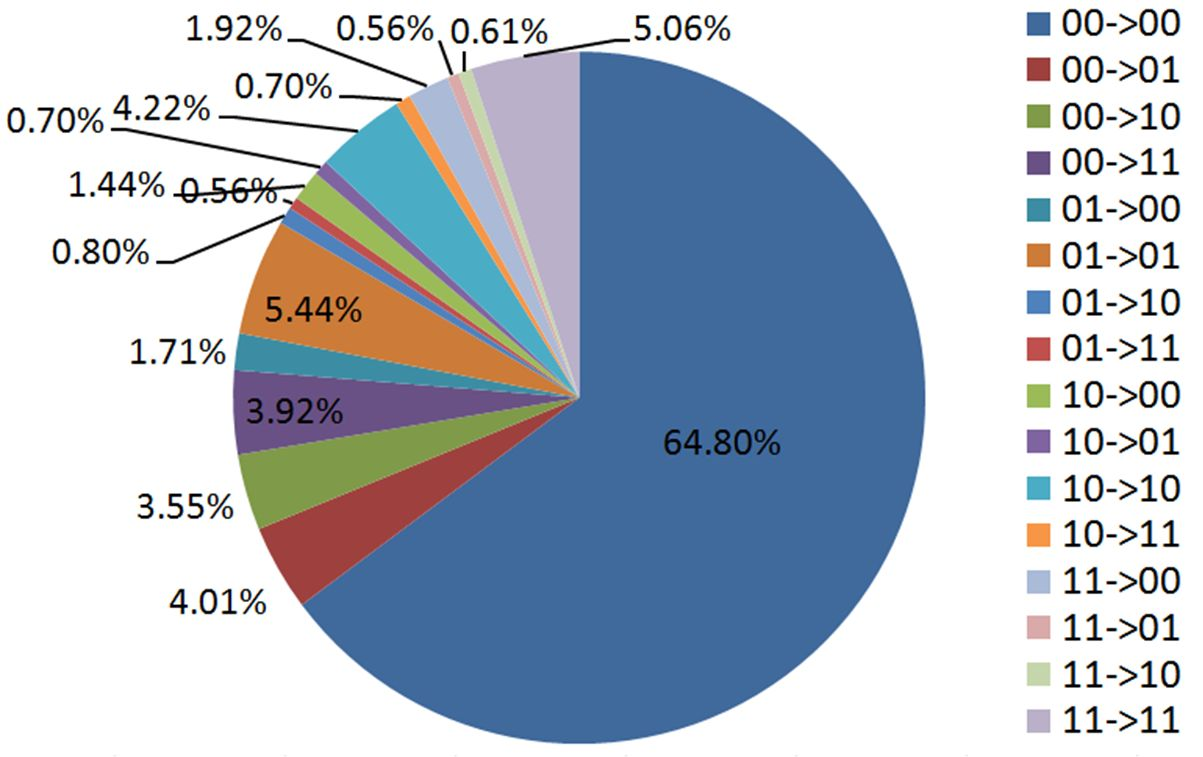
\includegraphics[width=0.5\textwidth]{./figure/mlc-tran.jpg}
\caption{The transition distribution between the different values of MLC MRAM bit}\label{mlc-tran}
\end{wrapfigure}

Multi-level cell (MLC) can effectively improve the integration density of memory by storing more than one bit information in a single memory device: $n$ bits are represented by  $2^n$ states of a storage device. MLC technology has achieved significant commercial success in NAND flash memory~\cite{Park04} and it has been explored in PCRAM~\cite{Raoux08,Bedeschi09}, STT-RAM~\cite{Lou08}, and RRAM~\cite{Baek05}. It can effectively improve the integration density of memory. However, the write endurance is also degraded due to the smaller resistance gap between two adjacent states.

Figure~\ref{mlc-tran} shows the transition distribution between the different logic values of 2-bit MLC in an in-order microarchitecture. We noticed that most of transitions occur between the same values, and hence, there is no need to change resistance state at all. Therefore, ``write-after-read'' scheme, which conducts only the necessary transitions based on the values of the new data being written and the original data stored in the MLC bit, could be the most efficient way for energy saving and lifetime improvement. Furthermore, we observe that the resistance switching in MLC need follow specific sequence. For example, the free layer of the MTJ in an MLC MRAM has two magnetic domains whose magnetization directions can be switched separately. The magnetization direction of \emph{soft domain} can be switched alone by a small current, while that of \emph{hard domain} can be switched by only a large current which is always associated with the magnetization direction switching of soft domain. Corresponding to the four resistance states -- $R00$, $R01$, $R10$, and $R11$ from low to high, an MLC MRAM cell may have total of $4! = 24$ encoding schemes for its four logic states -- $L00$, $L01$, $L10$, and $L11$. As we stated above that the probability of MTJ breakdown has an exponential relationship with the current amplitude through it, the hard domain switching can induce more damage on MTJ material than the soft domain switching. Properly selecting the encoding scheme of logic vs. physical states to reduce the hard domain switches based on the transition distributions can further improve the write endurance and lifetime of MLC MRAM.


\subsubsection{Process Variation-Tolerant Design}

As the process technology scales, device parameter fluctuations induced by process variations such as line-edge roughnesses (LERs) and oxide thickness fluctuations (OTFs) have become critical issues in affecting the performance of devices~\cite{Asenov03}. Similar to any other memory manufactured in the scaled technologies, emerging nonvolatile memories also suffer from the large process variation. For example, MTJ resistance increases exponentially with the thickness of oxide barrier between two magnetic layers. It was reported in~\cite{Tehrani00} that MTJ resistance increases by 8\% when the thickness of oxide barrier changes from 14${\AA}$ to 14.1${\AA}$. Moreover, the MTJ resistance variation will be aggravated by the further reduction of oxide barrier thickness in scaled technologies. Besides oxide barrier thickness, MTJ resistance is also significantly affected by the large MTJ geometry variations.

\paragraph{Read Failure}
%Strictly speaking,
Most of the emerging NVM technologies, e.g., MRAM and PCRAM, use device resistance as the data storage media. \textbf{Figure xxx(a)} illustrates a conventional voltage sensing scheme: Comparing the bit line voltage $V_{BL}$ generated by the selected memory cell with a reference signal $V_{REF}$ produced by the dummy cell. Ideally the resistance of the dummy cell should be set in the middle of the high and low resistance states ($R_H$ and $R_L$) of the selected memory cell. When $V_{BL}$ is higher than $V_{REF}$, the data storage device in the memory cell is in $R_H$ state, and vice versa. Usually a dummy cell is shared by multiple memory bits to reduce overhead. In reality, process variation incurs the resistance distribution of data storage device in memory cell as well as the dummy cell. As illustrated \textbf{Figure xxx(b)}, when the resistance variation $\sigma_R$ is large, the tails of $R_H$ or/and $R_L$ could be overlapped with $R_{dummy}$ and lead to the false detection of the stored value. We called it as \textbf{\emph{Read Failure}}.

Read failure is a severe problem in STT-RAM design for two main constraints. (1) The difference between two resistance states of MTJ is fairly small: $\Delta$R=$R_H-R_L$ $\approx$ $1000\Omega$ at 45nm technology node~\cite{Li09}; and (2) the MTJ resistance variation $\sigma_R$ is relatively high because it is extremely difficult to control oxide barrier thickness within a small range of variation, i.e. $0.5{\AA}$~\cite{Jeong03}. Besides the regular yield improvement techniques, such as redundant column/row and ECC (Error Correction Code), a self-reference read-out scheme could be another effective way to fix read-failure problem.

The basic idea of a self-reference reading is to compare the stored data in a memory cell with a reference value written to the same cell. By limiting the comparison within one single STT-RAM cell, the impact of bit-to-bit variation of MTJ resistance can be avoided. Previously some self-reference schemes were used in toggle-mode MRAM design~\cite{Tanizaki06,Jeong03}. We also successfully utilized it in STT-RAM design~\cite{Li:147723}. These schemes are all ``destructive'' because the original value in memory cell is wiped out when writing the reference value into MTJ, and has to be recovered at the end of the read operation. Obviously it prolongs read latency and introduces reliability issue.

\begin{wrapfigure}{r}{0.4\textwidth}\centering \centering
\vspace{-18pt}
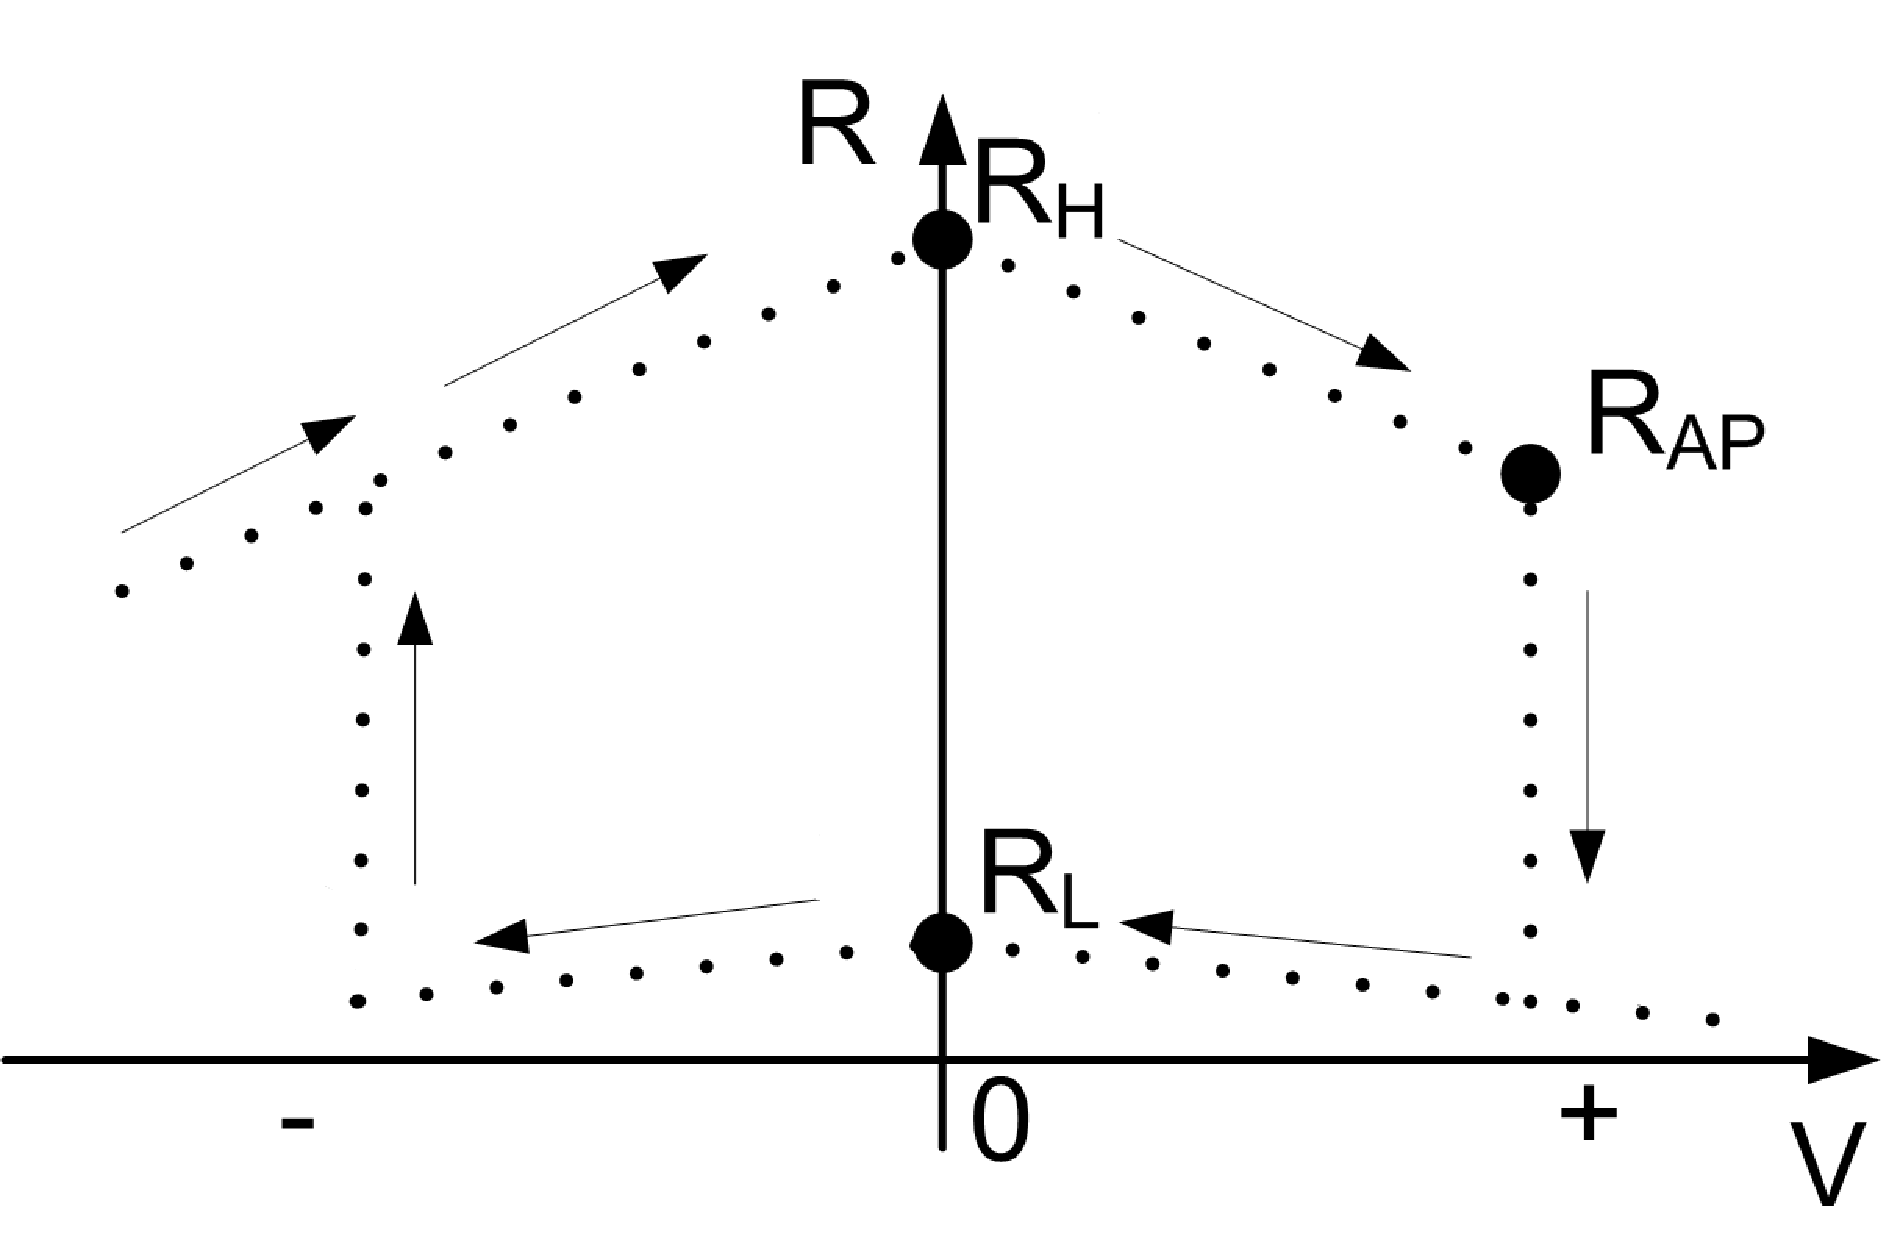
\includegraphics[width=0.4\textwidth]{./figure/RIcurve.pdf}
\caption{The static R-I curve of MgO-based MTJ. \textbf{\underline{HL: Modify Figure.}}}\label{mtj-RI}
\end{wrapfigure}

In this project, we will work on a \textbf{\textit{non-destructive self-reference}} methodology, which does not disturb the original data during read operations. The approach comes from the special R-I characteristic of MgO-based MTJ. As we can see in Figure~\ref{mtj-RI}, the MTJ current dependence of the high and the low resistance states are quite different: the current roll-off slope of high resistance is much steeper than that of low resistance. Therefore, we can sample the stored value of an MTJ twice by using two read currents $I_{R1}$ and $I_{R2}$ and compare the resistance difference ${\Delta}R=R1-R2$. Obviously ${\Delta}R_H$ is pretty big, while ${\Delta}R_L$ is close to `0'.

However, there are some uncertainties to realize this approach. For example, how much is the sensing margin in the new read-out scheme after considering process variations? What type of sensing circuitry is more optimal? Will a new sense-amplifier (SA) design be necessary? How does it impact memory array structure? How much yield improvement can be achieved with the new scheme? Will this scheme be still valid when technology further scales down? In this proposal we will investigate these issues and exploring the solutions. Our target is to minimize the effect of process variation and to improve read speed.

\paragraph{dopant drifting in Memristor, read window change???}
\textbf{\underline{HL: Add new section here.}}
Process has more impacts on memristor-based design, especially when memristor is used for a continuous data storage and detection.


\subsubsection{Density Enhancement}

Memory density is directly related to its capacity, and hence, reducing memory cell size and increasing density becomes an ultimate goal. In the past, technology scaling is always the biggest driving force to reduce single memory cell size by decreasing the pattern on chip. Process development plays an important role as well. For example, the charge storage materials of NAND Flash have gone through several generations to continue its scalability: from standard double polysilicon gate, to Silicon-Oxide-Nitride-Oxide-Silicon (SONOS), to bandgap engineered SONOS, and to TaN/Al$_2$O$_3$/SiN/SiO$_2$ (TaNOS)~\cite{Lu09}. The emerge of new NVMs is another good example to show the power of technology. On top of it, we should note that cell structure and circuit design technique can also constraint or boost memory density.

\paragraph{MRAM and PCRAM}

In a random access memory cell, usually an NMOS transistor is used as selection device (e.g. DRAM, MRAM and PCRAM) by connecting it in series with the data storage element. Such a cell structure needs three sets of terminals -- word line (WL), bit line (BL) and source line (SL). The routing requirement and design rules determine that the minimal possible cell size is 12$F^2$~\cite{Li09}. Here, $F$ represents the technology feature size.

The real memory size is also determined by ...
The real cell size could grow when the storage device cannot fit into it or the select transistor need serve as driving device too.



\paragraph{RRAM and Memristor}

Theoretically, the smallest memory cell is 4$F^2$, which has only two terminals -- one is horizonal (WL) and another is vertical (BL). The storage element is built at the cross-point of two metal wires, so it is called cross-point structure. RRAM can support data access in this structure by properly controlling the voltages applied on WL's and BL's. Moreover, the cross-point structure can grow in third dimension and forms an intra-die stacking structure. The memory storage cell is located in between any two adjacent metal layers which are used as interconnects. Within the same die size, the multiple memory layers further improve the memory density. Hence, RRAM is expected to replace NAND Flash memory as main storage in near future~\cite{ITRS07}.

From design point of view, RRAM technologies can be divided into two operation types: unipolar switching and bipolar switching. Unipolar operation executes the programming/erasing by using short and long pulse, or by using high and low voltage with the same voltage polarity. Usually a diode is served as selection device (1D1R). The data in bipolar switching RRAM can be changed by short voltage/current pulses with opposite voltage polarity. For such memory structures, non-ohmic device (NOD)~\cite{Yan4430255} is used to provide two-direction driving current as well as support process integration of cross-point structure. We call it as 1NOD-1R (See Figure~\ref{RRAM2}).

However, 1D1R and 1NOD-1R cell structures are facing on some design difficulties due to process limitation. Conceptually, NOD can be understood as two parallel connected diodes. Ideally, it turns on only when the voltage drop between the two terminals exceeds its threshold. However, the I-V characteristic curve of real device could be quite different.
%(See Figure~\ref{NOD}. Please note that the curves are not in the same scale.)~\cite{Yan4430255}.
This results in sneak path which has three or more cells in series as shown in Figure~\ref{RRAM2}(b). The sneak current can introduce disturbance on unintended cells during read, write and erase operations. Therefore, diode (P-N or Schottky) is more favorable as a selective element for RRAM array and intra-die stacking. However, it is extremely difficult to achieve the high quality diode with large $I_{on}$/$I_{off}$ ratio (large forward current $I_{on}$ and extremely small reverse current $I_{off}$) by using temperature limited BEOL (back end of line) process ($<400 ^{\circ}C$)~\cite{Sun:147791}.



\begin{figure}\centering
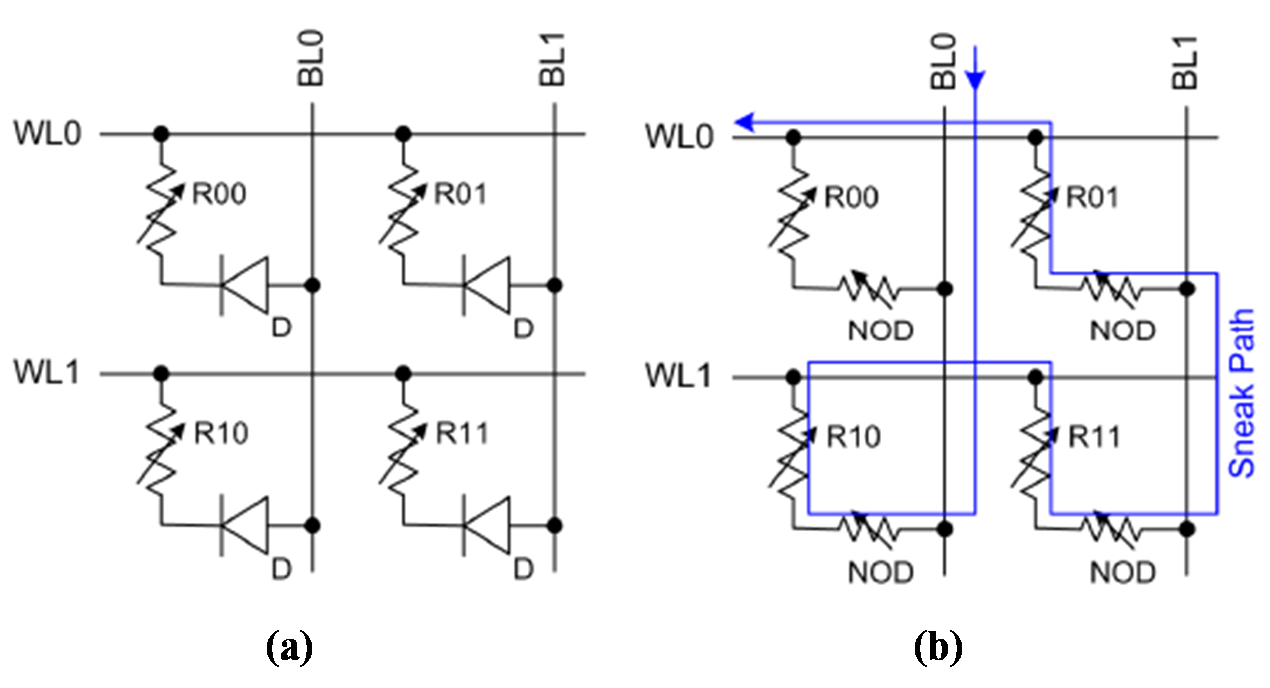
\includegraphics[width=0.50\textwidth]{./figure/HL-RRAM2.png}
\caption{RRAM memory cell scheme. (a) 1D1R; (b) 1NOD-1R.}\label{RRAM2}
\end{figure}




\paragraph{Using bipolar PMC as the selective element.} We propose to bipolar resistive switching devices as the selection device. Programmable-metallization-cell (PMC) could be a good candidate. PMC~\cite{Kozicki05} is a promising bipolar RRAM technology, which is composed of two solid metal electrodes -- relatively, one is inert and the other is electrochemically active. Between the two electrodes locates a thin electrolyte film. When a negative bias is applied to the inert electrode in programming operation (SET), metal ions in the electrolyte together with those flew from the positive active electrode can be reduced by the inert electrode. As a result, the metal ions form a small metallic ``nanowire'' between the two electrodes, which produces a low resistance. In erasing operation (RESET), a positive bias is applied on the inert electrode. Metal ions migrate back into the electrolyte and eventually to the negatively-charged active electrode. The ``nanowire'' is broken and the resistance increase back. The I-V curve is illustrated in Figure~\ref{PMC}(a). A higher voltage is required in RESET operation ($V_r$) than the one in SET operation ($V_s$).


\begin{comment}
\begin{figure}\centering
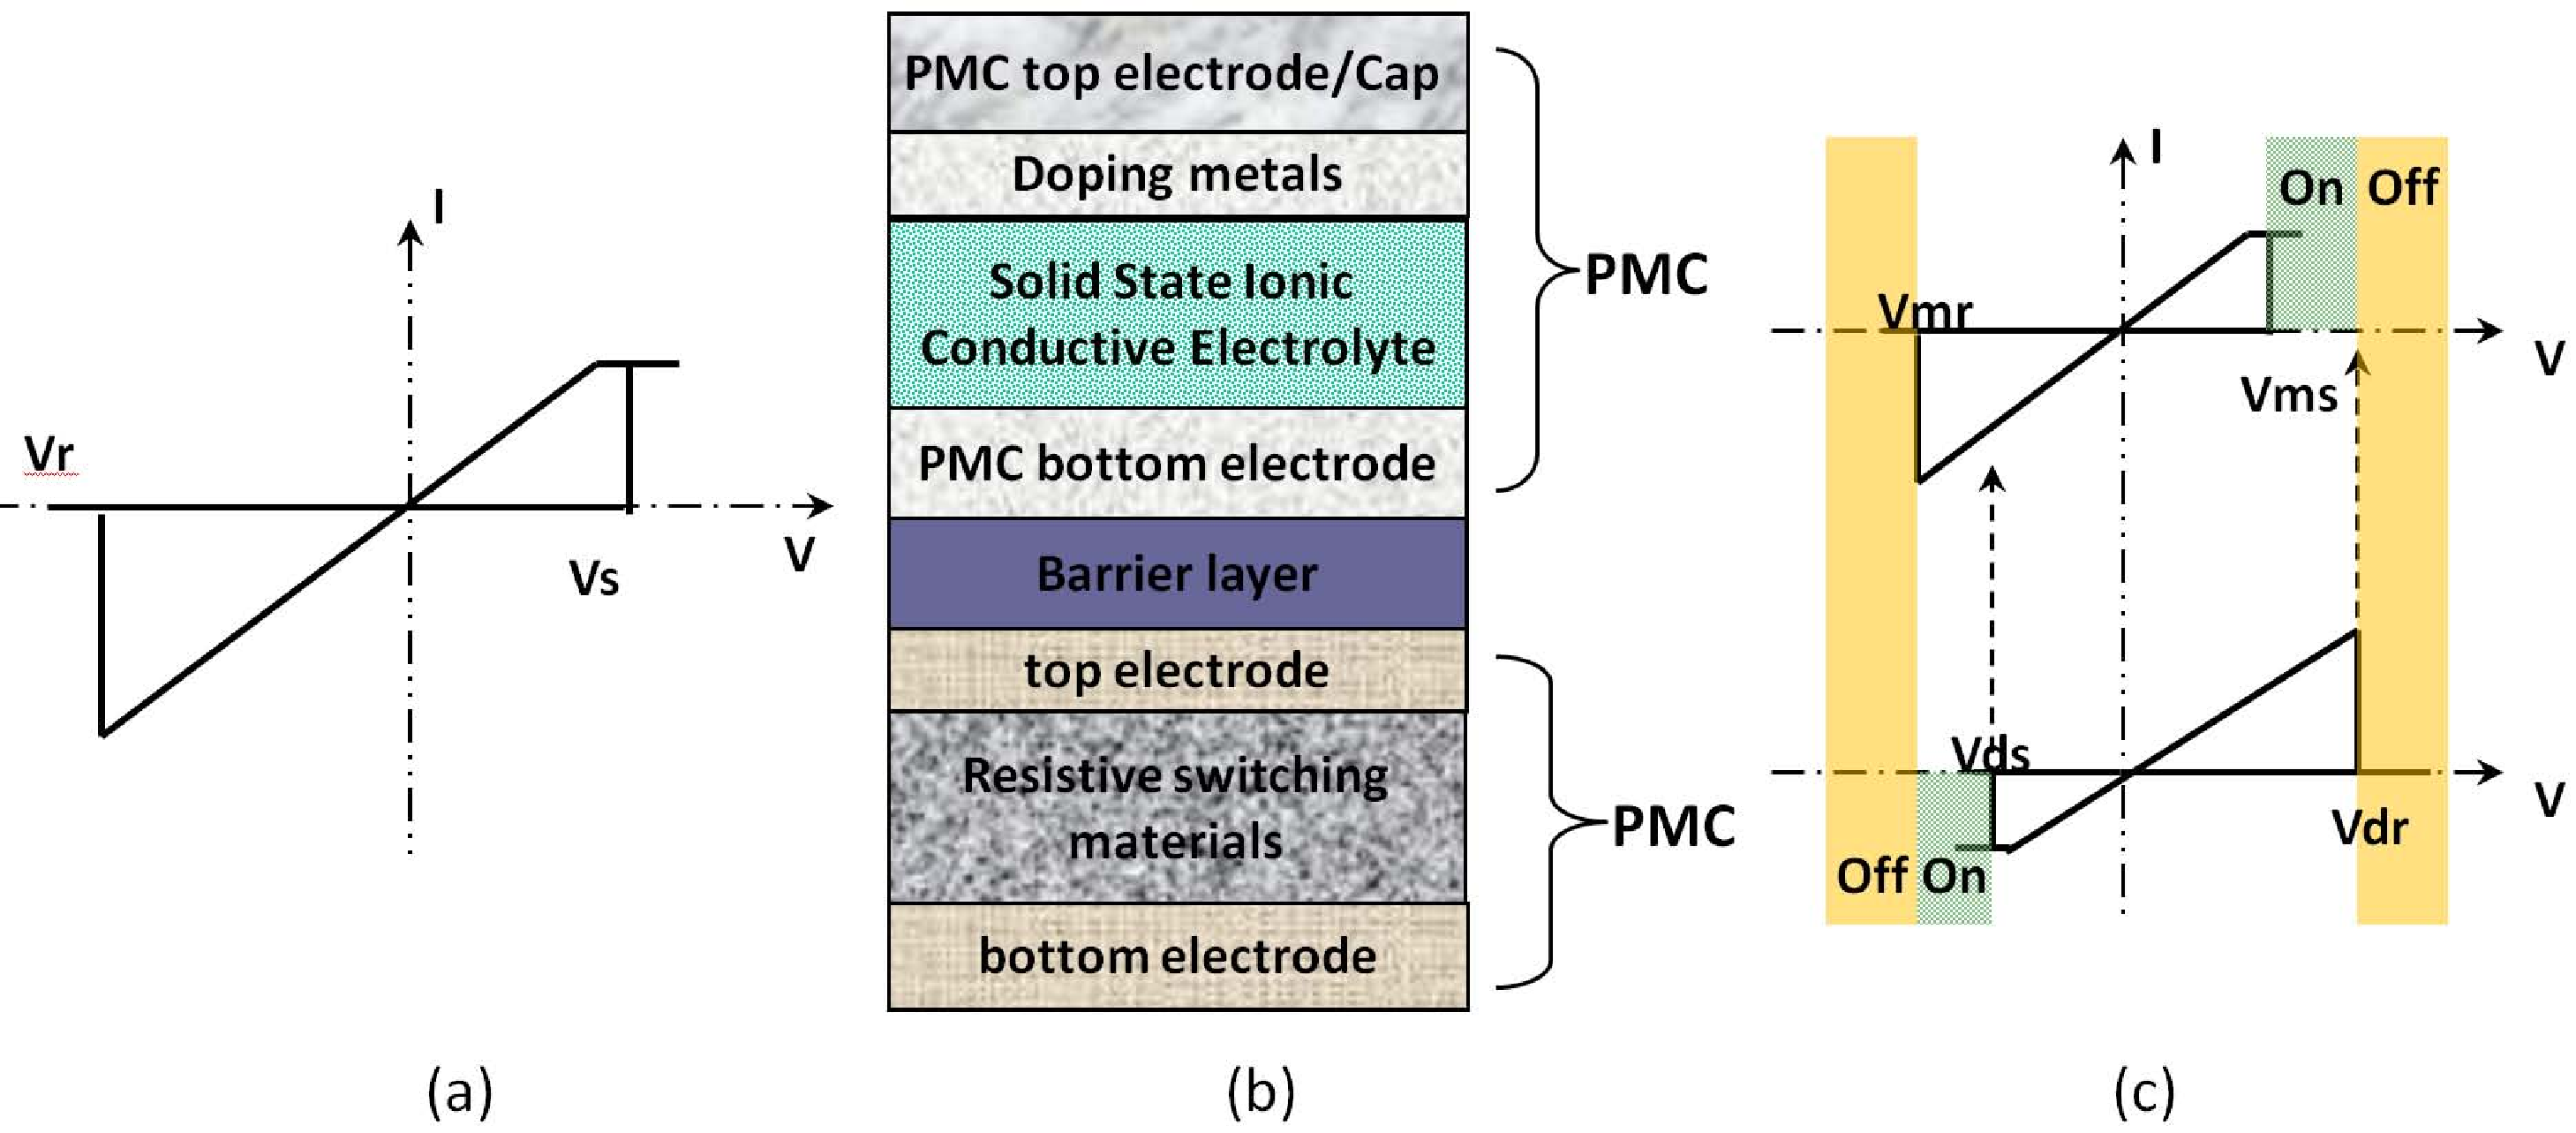
\includegraphics[width=0.75\textwidth]{./figure/PMC.png}
\caption{(a) I-V curve of PMC; (b) The proposed double cell configuration based on PMC technology; (c) I-V curves of the two back-to-back PMC devices shown in (b).}\label{PMC}
\end{figure}

\paragraph{Preliminary results:} Figure~\ref{PMC}(b) demonstrates a double cell configuration built by stacking two PMC's back to back with a barrier layer in between. In this structure, the PMC with active electrode on top is used as data storage (RRAM), while the main function of the PMC with active electrode at bottom is the selective device. This cell structure has been successfully demonstrated in process~\cite{Sun:147791}. Since PMC technology itself is compatible to CMOS process, the integration of the proposed structure is friendly to CMOS technology too.

The operations can be explained by using the corresponding I-V curves of the two PMC devices shown in Figure~\ref{PMC}(c). Here, the top and bottom I-V curves are for the memory and selection devices, respectively. We can see that when the voltage drop cross the RRAM cell exceed $V_{r}$, the RRAM cell is ``off'' because either PMC1 or PMC2 are in high resistance state.
\begin{itemize}
  \item SET operation: First, a negative bias in between $-V_{ds}$ and $-V_{mr}$ is applied to turn on the switch; Then a positive voltage higher than $V_{ms}$ but smaller than $V_{dr}$is used to program memory. After data is successfully written to the cell, further increase voltage to higher than $V_{dr}$ in order to turn off the switch.
  \item RESET operation: Apply a negative bias lower than $-V_{mr}$, it will first turn on the switch and than reset the memory cell. In such a situation, there is no way to turn off the switch.  But there is no leakage path either due to the high resistance of the memory.
  \item READ operation: Like SET and RESET, the switch needs to be turned on first by applying a negative bias in between $-V_{ds}$ and $-V_{mr}$. Then a small current can be used to read memory cell resistance state.  At the end of the read operation, the switch is required to turned off or keep it on when memory is in low or high resistance state, respectively.
\end{itemize}
\end{comment}

Compared to diode or NOD, PMC based switch has two advantages -- bipolar switching and large $I_{on}$/$I_{off}$ ratio. Hence, the proposed scheme could be used in bipolar switching RRAM design with minimized sneak current. Although we have investigate the feasibility based on theoretical analysis, there are still a lot of unsolved issues. For example, how to control timing and applied voltage? What kind of peripheral circuitry floorplan will be optimal for the proposed RRAM design? And again, how will process variations affect the proposed RRAM scheme? In this project, we will address these circuit issues from both device and circuit point of views and explore the solutions.


\subsubsection{Preliminary results and Collaborations:}
Previously, we have already successfully utilized the destructive self-reference scheme in STT-RAM design~\cite{Li:147723}. The feasibility of the non-destructive self-reference scheme has been also discussed and analyzed in theory~\cite{Chen:147727}.
Add experience on SRAM design??
